\chapter{Timing Characteristics of the Program}\label{ConnectingBreakoutBoard} 
\textbf{Name: Group 630}\\
\textbf{Date: 11/05 - 2016}

\subsubsection{Purpose}
Check the proper behavior of the program running on the microcontroller to ensure proper operation of the control system.

\subsubsection{Setup}
\begin{figure}[H]
  \centering
  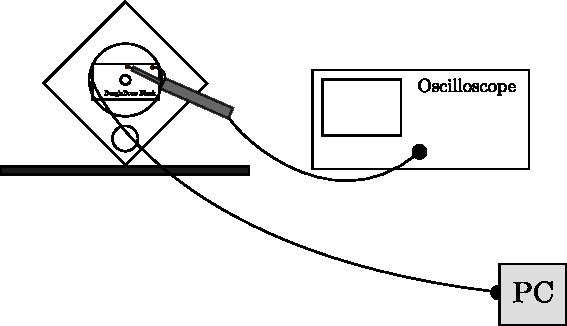
\includegraphics[scale=1]{figures/programTimingSetup}
  \caption{Setup diagram}
  \label{LabSetupRangeTest}
\end{figure}
\fxnote{Modify picture to probe on the BBB}
To measure timing characteristics, it is necessary to connect to external pins of the BeagleBone Black and raise and lower the pin around the interesting program area in the source code. Here, the section of interest is the whole function \lstinline{runController()} which performs the sensor readings and runs the controller computations.\\
It should be made sure that the current sent to the motor controller is null, so that the wheel stands still while doing the measurement.

\subsubsection{List of Equipment}
\begin{table}[H]
  \begin{tabular}{|l|l|p{4.3cm}|}
    \hline%------------------------------------------------------------------------------------------------------------
    \textbf{Instrument}                                   &  \textbf{AAU-no.} &  \textbf{Type}            \\
    \hline%------------------------------------------------------------------------------------------------------------
    Oscilloscope                                          &  3386             &  Agilent 54621A           \\
    \hline%------------------------------------------------------------------------------------------------------------
    Dedicated Power Supply of Cubli \small{(24 V - 3 A)}  &                   &  XP Power, AEB70US24      \\
    \hline%------------------------------------------------------------------------------------------------------------
    Probe                                                 &                   &  1:1                      \\
    \hline%------------------------------------------------------------------------------------------------------------
      Computer                                            &                   &  Asus UX301LA  \\
    \hline%------------------------------------------------------------------------------------------------------------
  \end{tabular}
\end{table}

\subsubsection{Procedure}
\begin{enumerate}
  \item Make the setup with connections as seen on \figref{LabSetupRangeTest}, with ground on pin 2 and signal on pin 26 of the P8 header on the BeagleBone Black.
  \item Launch the appropriate program over a USB SSH connection.
  \item Set the oscilloscope on rolling and calibrate it so that a few periods of the pulse signals can be clearly seen on the display.
  \item Stop the acquisition and save the data to a floppy-disk as a CSV file. Gather the CSV log file generated by the program, from the BeagleBone Black.
\end{enumerate}

\subsubsection{Results}
\begin{figure}[H]
  \centering
  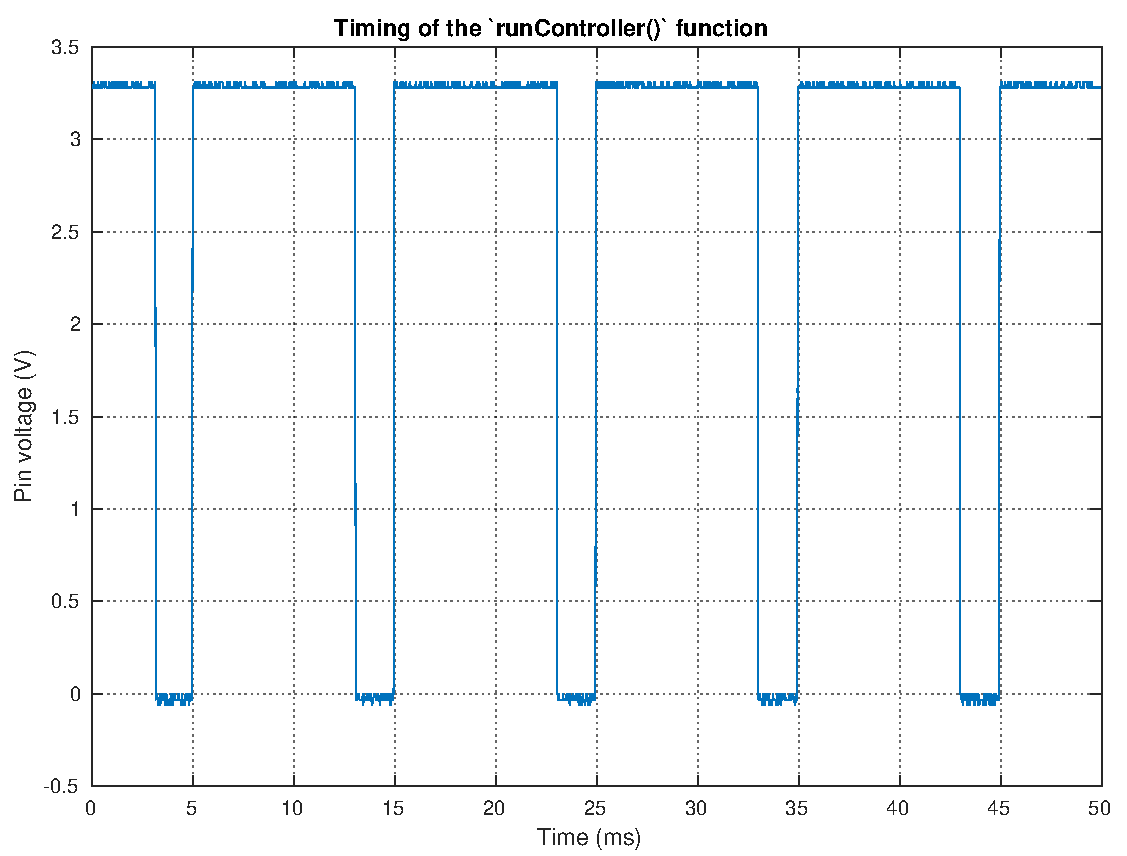
\includegraphics[scale=0.6]{figures/programTiming}
  \caption{Pulse signal of the monitored code region executing the main controller operations.}
  \label{fig:programTiming}
\end{figure}
\Figref{fig:programTiming} shows that the function \lstinline{runController()} which runs the main operations of the controller as well as the sensor readings, is called every \SI{10}{ms} along the few periods shown on the graph. This is the expected behavior since the function runs in a scheduled thread and it seems to respect, rather precisely, the timing period it is asked in the code to run at.\\
It is also interesting to note that each call made to the function lasts approximately \SI{8}{ms} which means this critical section of the code has the time to run completely before the next call. However, this does not leave a very large margin to add other potential features in this code environment.\\
By running a few other similar tests and removing parts of the code, the sensor readings are identified to be the most time consuming feature. Furthermore, jumps in the potentiometer readings, which can be seen on \figref{fig:potMeterJumps1} and \figref{fig:potMeterJumps2} seem to arise from the way the ADC values are read by the program through the operating system's I/O system. The area at issue in this situation seems identifiable, but since it is decided to eliminate the potentiometer in this project, and since the measured data is only negligeably affected in any case, no further investigation is to be made on this matter during this project.

\begin{minipage}{0.45\linewidth}
  \begin{figure}[H]
    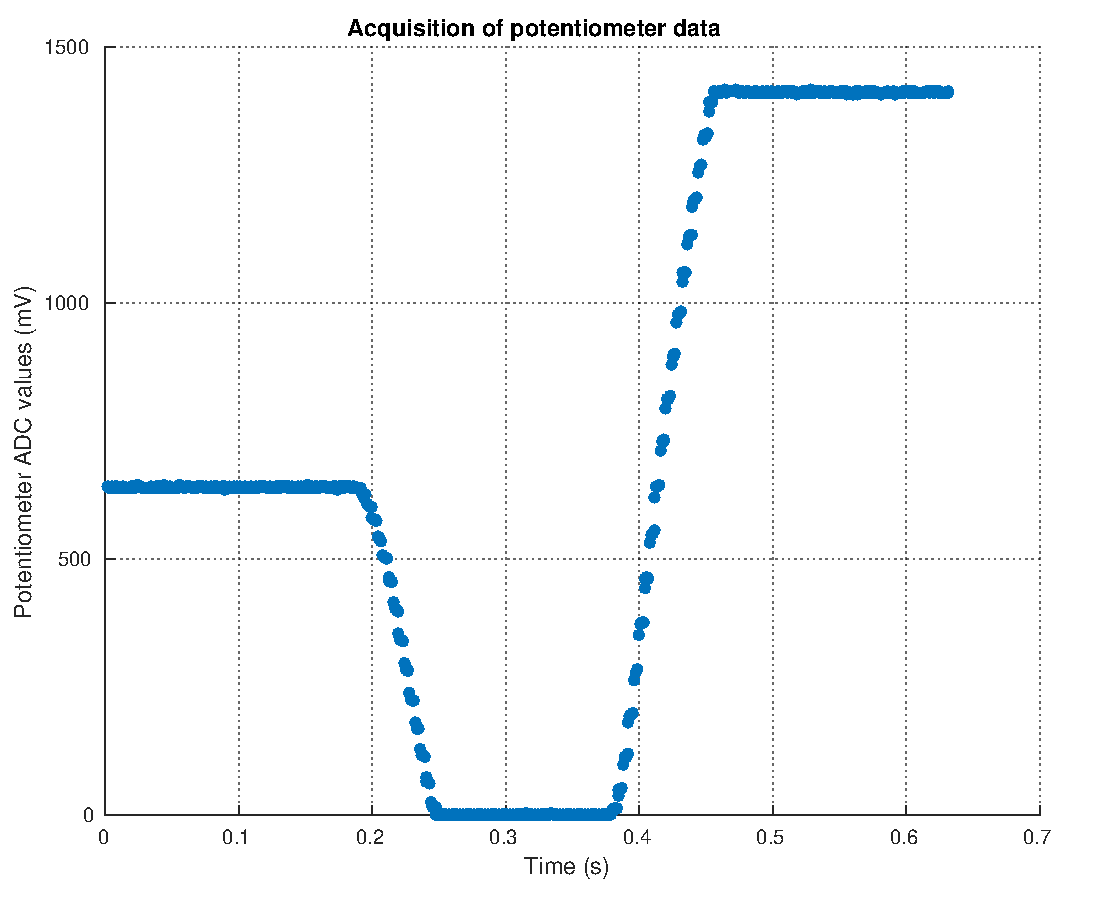
\includegraphics[scale=.48]{figures/potMeterJumps1}
    \captionsetup{justification=centering}
    \captionof{figure}{Potentiometer readings from a range test. Groups of data points can be observed.}
    \label{fig:potMeterJumps1}
  \end{figure}\vspace{-5mm}
\end{minipage}
\hspace{0.03\linewidth}
\begin{minipage}{0.45\linewidth}
  \begin{figure}[H]\vspace{-4mm}
    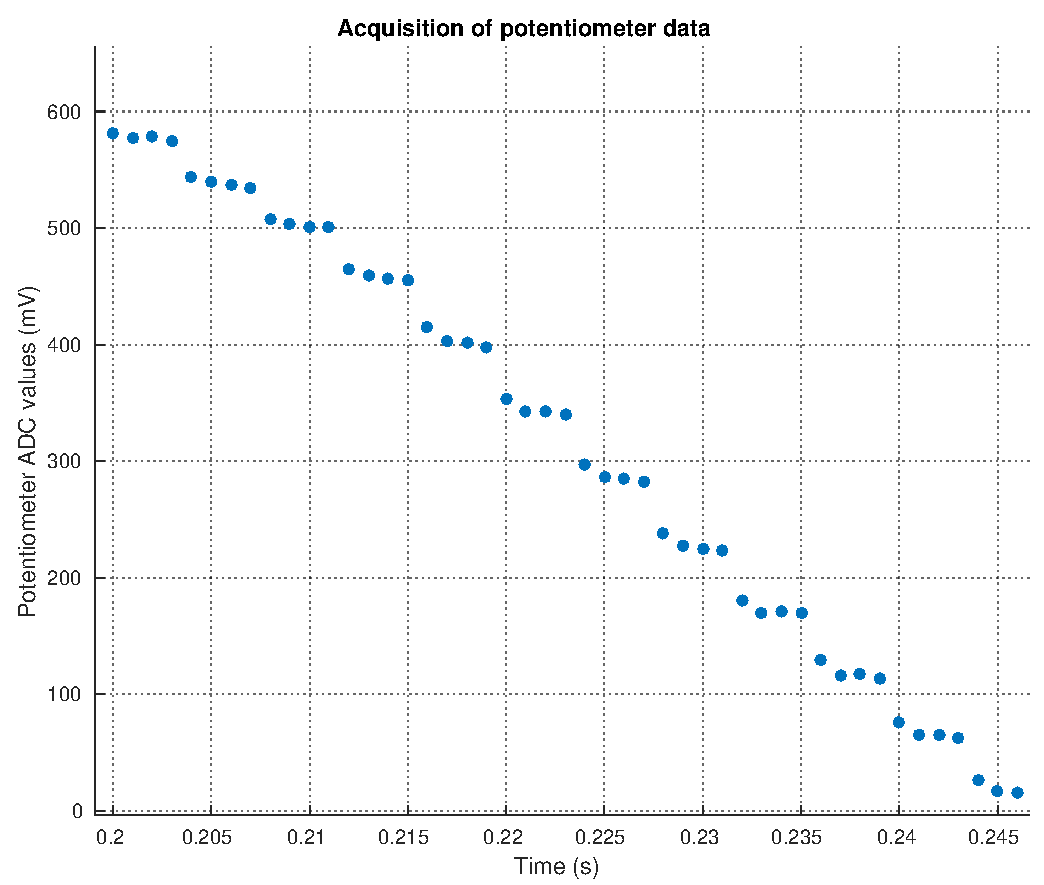
\includegraphics[scale=.48]{figures/potMeterJumps2}
    \captionsetup{justification=centering}
    \captionof{figure}{Zoom-in on the potentiometer readings. Irregularities can be clearly seen in the ADC values.}
    \label{fig:potMeterJumps2}
  \end{figure}\vspace{-5mm}
\end{minipage}